bg
\section{Minding the Gap}
\label{sec:evaluation}

If achievable, coordination-freedom enables scalability limited to
that of available hardware: namely, server and network capacity. This
is powerful: a \cfree application can scale out without sacrificing
correctness, latency, or availability. However, this raises two
important questions: what happens if \cfreedom is not possible (i.e.,
\iconfluence does not hold), and how commonly can \cfreedom be
achieved? In this section, we begin to answer both of these questions
via both simple modeling and via a real-world, proof-of-concept
implementation of what is traditionally considered a challenging OLTP
benchmark. The former is the realm of traditional concurrency control,
while the latter offers a glimpse at what is attainable via
coordination-avoiding database systems, which coordinate only when
necessary.

\subsection{Costs of Coordination}

When an application is \iconfluent and therefore executable with
\cfreedom, scalability is effectively guaranteed: given an appropriate
execution plan, there is no fundamental reason why the application
cannot attain indefinite scale-out. We will shortly quantify these
benefits in a real-world system, but, for now, we evaluate the
alternative: what happens if a system must coordinate?

\begin{figure}
  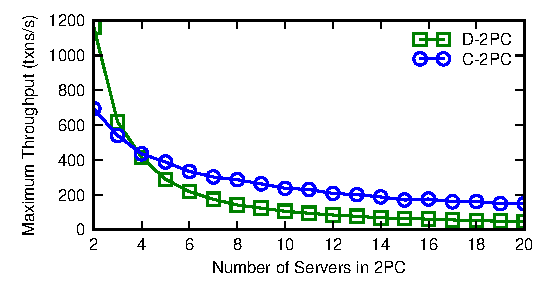
\includegraphics[width=\columnwidth]{figs/singledc-twopc.pdf}\\ {\centering
    \textbf{\scriptsize a.) Local-area network scenario based on
      traces from~\cite{bobtail}}\par}
  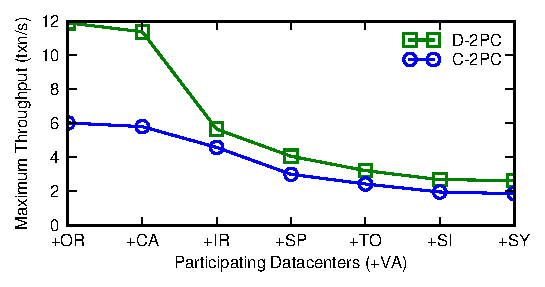
\includegraphics[width=\columnwidth]{figs/multidc-twopc.pdf}\\ \textbf{\scriptsize
    b.) Wide-area network scenario based on traces
    from~\cite{hat-vldb} with transactions origininating from a
    coordinator in VA (VA:~Virginia, OR:~Oregon, CA:~California,
    IR:~Ireland, SP:~S\~{a}o Paulo, TO:~Tokyo, SI:~Singapore,
    SY:~Sydney)}

\caption{Atomic commitment latency as an upper bound on throughput
  over LAN and WAN networks.}
\label{fig:2pc}
\end{figure}

As studied in traditional database systems, one of the primary
challenges in scaling database systems to both multiple replicas and
across multiple partitions is the atomic commitment problem: if a
given transaction might abort, all servers it accesses (whether
replicas of the same item or replicas of different items) must agree
to unilaterally commit or abort the
transaction~\cite{bernstein-book}. This \textit{atomic commitment}
problem is well-studied in both the database and distributed systems
literature, with many variants including two-phase commit,
decentralized two-phase commit, and three-phase
commit~\cite{atomictransactions,paxos-commit,traiger-tods}. For each
pair of conflicting transactions, the servers responsible for the
conflicting operations must choose which (if either) should commit
(and, in database systems, is often coupled with a decision about the
commit order~\cite{hat-vldb,calvin,traiger-tods}). Regardless of
implementation technique, if multiple servers participate in the
commit decision (e.g., locking across partitions or employing multiple
active validators), they must undergo atomic commitment (whereas a
single-server implementation would be limited in throughput to its
capacity). Therefore, the duration of atomic commitment determines the
the maximum achievable throughput for modifications to a given data
item. If atomic commit take $10$ms, then, for abortable updates, we
can achieve throughput of $100$ transactions per second per item. Of
course, there are many possible optimizations to this simple rule of
thumb, including batching and reordering of
commits~\cite{calvin}. Moreover, given non-conflicting transactions,
aggregate system throughput can be much higher than the per-item
throughput limitations~\cite{spanner, f1}. However, for arbitrary
schedules of transactions, atomic commitment latency is a reasonable
upper bound on per-item throughput for conflicting, distributed
operations.

To better understand the relationship between atomic commitment
(necessitated by non-\iconfluent, abortable transactions) and
scalability, we performed a simple analysis of achievable throughput
using recently published datasets of real-world communication delay
from both local-area~\cite{bobtail} and wide-area~\cite{hat-vldb}
networks. We use Monte Carlo analysis to determine the latency of
traditional two-phase commit~\cite{bernstein-book} (\dpc) and
decentralized two-phase commit~\cite{paxos-commit} (\cpc). We consider
groups of increasing numbers of participants and assume that
transactions are perfectly pipelined such that each participant
\texttt{prepare}s the next transaction immediately after it has
\texttt{commit}ted the prior transaction. Therefore, two-phase commit
requires two message delays ($N$ \textit{prepared} messages from all
nodes to a ``coordinating'' participant and $N$ messages to send the
\texttt{commit} response), while three-phase commit requires one
message delay ($N^2$ messages in an all-to-all broadcast of
\texttt{prepared} messages). We strictly consider network latency
(i.e., local processing time incurred by locking, latching,
validation, or I/O delays would only increase latency).

Figure~\ref{fig:2pc} show our results for both local-area
(\ref{fig:2pc}a) and wide-area (\ref{fig:2pc}b) networks.  In the
local area, with only two servers participating in atomic commitment
(e.g., replication factor of $2$ or, alternatively, two conflicting
operations on items residing on different servers), we see a maximum
attainable throughput of approximately $1100$ transactions per second
(via \dpc; $750$/s via \cpc). With ten servers participating, \dpc
throughput drops to only $120$ transactions per second (resp. $200$
for \cpc): the long-tail of network latency surfaces as the number of
messages sent increases. In the wide area, the effects are stark: if
only coordinating within the continental US from Virginia to Oregon,
\dpc message delays incur a latency of around $83$ milliseconds per
commit, resulting in a throughput of $12$ operations per second. If
coordinating between all eight EC2 availability zones, throughput
drops to slightly over $2$ transaction per second in both algorithms.

While this study is based solely on reported latencies, deployment
reports corroborate our findings. For example, Google's F1 uses
optimistic concurrency control via WAN with commit latencies of
$50$ to $150$ms. As the authors discuss, this limits throughput to between
$6-20$ transactions per second per data item~\cite{f1}. Megastore's
average write latencies of $100$ to $400$ms suggest similar throughputs to
those that we have predicted~\cite{megastore}. Indeed,
\textit{aggregate throughput} may be substantially greater as multiple
2PC rounds for disjoint sets of data items may safely proceed in
parallel. However, \textit{worst-case} access patterns will indeed
greatly limit scalability: as many before us have noted, adding more
active servers/replicas in non-\cfree models like serializability can
greatly reduce throughput~\cite{abadi-vll,calvin,jones-dtxn}.

\subsection{Proof of Concept}

As a proof of concept application of \cfreedom analysis, we next show
that the classic benchmark for OLTP performance is not particularly
challenging from a distributed coordination perspective. The TPC-C
benchmark is often used as the gold standard for database concurrency
control both in research and in industry~\cite{tpcc}, and in recent
years has been used as a yardstick for distributed database
performance (e.g., Calvin~\cite{calvin}, H-Store~\cite{hstore},
Silo~\cite{silo}). Accordingly, we begin by determining the
fundamental scalability limitations of the backbone of this benchmark,
the New-Order transaction.

New-Order corresponds to the placement of an order in a wholesale
supplier application. Each new order randomly chooses a set of items,
decrements their stock, and records the order request in a designated
table. There are three challenging components of New-Order, which we
describe below:
\begin{itemize}

\item \textit{Foreign key constraints (Consistency Criteria
  3.3.2.\{4-7, 11\}).} New-Order requires maintaining foreign key constraints:
  when an order is recorded in the \texttt{ORDER} table, the
  corresponding orders for each item should be reflected in the
  \texttt{ORDER-LINE} table. Similarly, the new order in the
  \texttt{ORDER} table should be present in the \texttt{NEW-ORDER}
  table. In a traditional database system, we might use locks to
  atomically control the visibility of these updates to multiple
  tables. However, our SQL analysis tells us that we can maintain
  these constraints under insert with \cfreedom. Indeed, with the
  newly proposed \cfree ANON algorithm~\cite{ramp-txns}, we can ensure
  that all of these updates are visible, or none are.

\item \textit{Sequential ID assignment (Consistency Criteria
  3.3.2.2-3).} Each New-Order executed in a pre-determined
  per-warehouse requires a sequentially assigned ID (e.g.,
  \texttt{AUTO\_INCREMENT}). This poses a challenge: the
  \texttt{DISTRICT\_NEXT\_O\_ID} column must be incremented at the
  same time that corresponding rows are inserted into the
  \texttt{ORDER}, \texttt{NEW-ORDER}, and \texttt{ORDER-LINE}
  tables. We know from our SQL analysis that this sequential
  assignment is not \cfree, so, for a compliant run, we will need to
  coordinate (others forego this sequential
  constraint~\cite{hat-vldb,silo} at the expense of compliance). A
  strawman approach would hold locks for the duration of each
  New-Order, but this greatly reduces throughput. We wait to assign
  the district's next ID until commit time. When inserting rows into
  the \texttt{ORDER}, \texttt{NEW-ORDER}, and \texttt{ORDER-LINE}
  tables, the database assigns a temporary, uniquely generated key
  and, upon commit, adds a reference (in a separate table) that
  resolves this temporary key to point to the true sequential
  key. Accordingly, the database only holds locks for a single atomic
  increment of the district ID counter.

\item \textit{Materialized view maintenance (Consistency Criteria
  3.3.2.\{1, 8-10, 12\})}. Throughout transaction execution, a variety
  of materialized counters should be maintained (e.g., \texttt{W\_YTD
    = sum(D\_YTD}). With appropriate counter data types as in
  Section~\ref{sec:merge}, these constraints are all achievable with
  \cfreedom.
\end{itemize}

All told, TPC-C New-Order coordination can be limited to a single,
atomic increment-and-get operation on each district's order sequence
number. Our \cfreedom analysis shows that ten of twelve required
constraints are achievable without synchronous coordination and the
remainder (3.3.2.2-3) are satisfiable via non-abortable single-site
operation. Hence, scalability for a single warehouse is limited to
atomic increment-and-get on a single machine. Indeed, when we execute
the above query plan on a linearizable main-memory database prototype
(Figure~\ref{fig:clients}; we disregard think time and per-warehouse
client limits, as is
standard~\cite{calvin,hstore,abadi-vll,jones-dtxn}), we indeed
bottleneck on sequence number assignment. On EC2 cc2.8xlarge
instances, as depicted, we achieve over $12K$ New-Order transactions
per second per warehouse. Deploying multiple warehouses per server
decreases contention and we attain throughput in excess of $17K$
transactions per second before bottlenecking on CPU. There is no
synchronous coordination across partitions, so varying the percentage
of distributed transactions results in a modest ($25\%$) throughput
reduction due to CPU utilization due to serialization and the kernel's
TCP/IP stack (Figure~\ref{fig:pct}). In contrast, traditional
(serializable) approaches (as Figure~\ref{fig:2pc} hints) incur
throughput overheads ranging from 66--88\%~\cite{abadi-vll}.

\begin{figure}
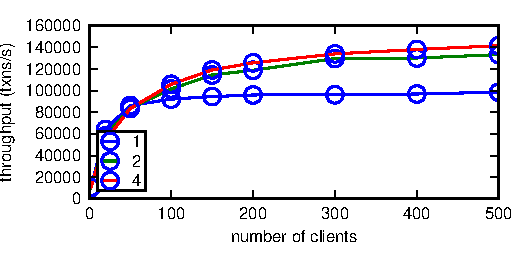
\includegraphics[width=\columnwidth]{figs/wh_thru.pdf}\vspace{-1em}
%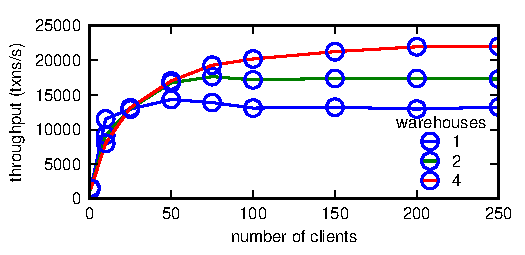
\includegraphics[width=\columnwidth]{figs/wh_thru_single.pdf}
\caption{TPC-C New-Order throughput across eight servers.}
\label{fig:clients}
\end{figure}

\begin{figure}
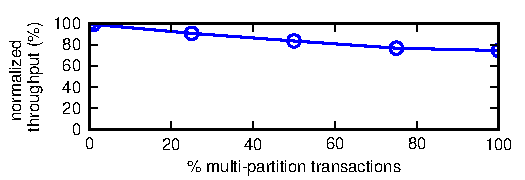
\includegraphics[width=\columnwidth]{figs/pct_thru.pdf}\vspace{-1em}
\caption{Coordination-free distributed execution of TPC-C New-Order
  (primary cost: CPU overhead due to serialization).}
\label{fig:pct}
\end{figure}

Unsurprisingly, a coordination-avoiding strategy allows linear scaling
to 100 machines (Figure~\ref{fig:scaleout}). On a cluster of 100 EC2
cc2.8xlarge servers spanning three \texttt{us-west} availability zones
($5$ warehouses per server), we achieve over 1.6 million New-Order
transactions per second. We achieve 89.5\% of perfect scaling from one
to 100 machines and perfect scaling from ten to 100 machines. At peak,
each server is CPU bound due to our current, admittedly fairly
inefficient implementation. Nonetheless, in a scale-out system,
single-node performance tuning is dwarfed by the power of
coordination-avoiding operations. A comparison with a system providing
serializability or even Snapshot Isolation would be unfair, but we are
unaware of any other compliant TPC-C implementation that achieves
greater than $500K$ New-Order transactions per second (e.g., Oracle
11G, Calvin~\cite{calvin}, Silo's non-FastIDs~\cite{silo},
VLL~\cite{abadi-vll}). In contrast, we present these results as a
proof of concept that executing even ``challenging'' workloads like
TPC-C that contain many complex integrity constraints are not at odds
with scalability if implemented in a coordination-avoiding manner.

\begin{figure}
\begin{center}
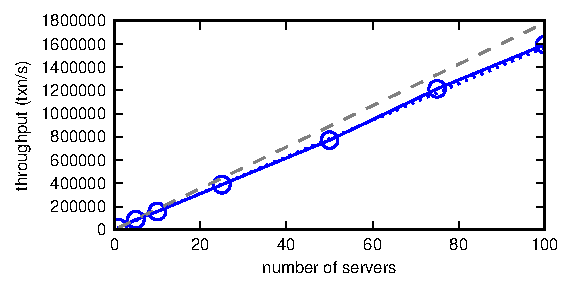
\includegraphics[width=\columnwidth]{figs/thru_scale.pdf}\vspace{-2em}
\end{center}
\caption{Coordination-free distributed execution of TPC-C New-Order is
  linearly scalable (dashed line is perfect scaling).}
\label{fig:scaleout}
\end{figure}

\minihead{Additional transactions} We have focused here on New-Order
as it is the subject of considerable attention and is the only
distributed transaction in the benchmark. However, the remainder of
the TPC-C transactions are largely uninteresting from the perspective
of coordination. We omit a full analysis, but all operations except
for the Delivery transaction are implementable via a combination of
foreign key updates and commutative counter increment/decrement, and
the Delivery transaction is easily implemented (as acknowledged in the
benchmark specification~\cite{abadi-vll}) as a single-partition
transaction. The TPC-C isolation requirements (reflecting the ANSI SQL
specification) are all achievable via client-side caching as proposed
by Bailis et al.~\cite{hat-vldb}.


\minihead{Additional applications} While TPC-C is the ``current
industry standard for evaluating the performance of OLTP
systems''~\cite{oltpbench}, we are aware that it may be a
simplification of real-world workloads. For greater variety, we
examined the transactions in the OLTPBenchmark suite~\cite{oltpbench}
and found that, in nine of fourteen remaining (non TPC-C) benchmarks,
the workload transactions did not involve integrity constraints (e.g.,
did not modify primary key columns), one (\texttt{CH-bencCHmark})
matched TPC-C, and two specifications implied (but did not explicitly
state) a requirement for coordination due to unique ID assignment
(\texttt{AuctionMark}'s \texttt{new-purchase}, \texttt{SEATS}'s
\texttt{NewReservation}; achievable like TPC-C New-Order). The
remaining two benchmarks, \texttt{sibench} and \texttt{smallbank} were
specifically designed as research benchmarks for serializable
isolation. The three ``consistency conditions'' in the newer TPC-E
benchmark (not in OlTPBenchmark) represent a subset of the twelve
conditions from TPC-C that we consider here. It is possible (and even
likely) that these benchmarks are simply under-specified, but,
according to official specification, TPC-C contains the most rigorous
coordination-intensive invariants among the benchmarks we encountered.

Anecdotally, our conversations with end-users have not identified
invariants that are radically different than those we have proposed,
and a simple thought experiment identifying the invariants required
for, say, a social networking site, are fairly simple (e.g., username
uniqueness, foreign key constraints between updates, privacy
settings). Nonetheless, we view the further study of real-world
invariants to be a necessary area for future investigation.


